\documentclass[11pt,a5paper]{article}

\usepackage[T1]{fontenc}
\usepackage[utf8]{inputenc}
\usepackage{lmodern, microtype}
\usepackage[estonian]{babel}
\usepackage{siunitx}
\sisetup{inter-unit-product=\ensuremath{{}\cdot{}}, per-mode=fraction, exponent-product=\cdot, output-decimal-marker={,}}
\usepackage{graphicx}
\usepackage{wrapfig}
\usepackage{adjustbox}
\usepackage{tikz}
\usetikzlibrary{arrows.meta, patterns, patterns.meta}
\usepackage{pgfplots}
\usepackage[european]{circuitikz}
\tikzset{component/.style={draw,thick,circle,fill=white,minimum size=0.75cm,inner sep=0pt}}
\usepackage{amsmath,amssymb}
\usepackage{amsfonts}
\usepackage[hidelinks]{hyperref}
\usepackage{csquotes}
\usepackage{caption}
\usepackage{enumitem}
\topmargin=-3.0cm \textheight=19cm \textwidth=12.9cm
\oddsidemargin=-1.5cm  \evensidemargin=-1.5cm
\setlength{\parindent}{0pt} \setlength{\parskip}{6pt} \sloppy
\sloppy \relpenalty=10000 \binoppenalty=10000
\pagestyle{empty}

\newcommand{\numb}[1]{\vspace{5pt}\textbf{\large #1}}
\newcommand{\nimi}[1]{(\textsl{\small \uppercase{#1}})}
\newcommand{\punktid}[1]{(\emph{#1~p.})}
\newcounter{ylesanne}
\newcommand{\yl}[1]{\addtocounter{ylesanne}{1}\numb{\theylesanne.} \nimi{#1} \newblock{}}
\newcommand{\autor}[1]{}% Kasuta võistluse ajal
% \newcommand{\autor}[1]{\emph{Autor: #1}}% Kasuta kui vaja autorit

\begin{document}
\begin{center}
  \textbf{\Large Eesti koolinoorte 71. füüsikaolümpiaad} \par
  \emph{6. aprill 2024. a.\\Gümnaasiumi ülesanded (10.--12. klass)}
\end{center}

\resizebox{\textwidth}{!}{
  \emph{%
    \begin{tabular}{@{}l@{}}
      \textbf{Palun kirjutada iga ülesande lahendus eraldi lehele.}\\
      Lahendamisaeg on 5 tundi. \\
      Iga osavõtja võib lahendada kõiki pakutud ülesandeid. \\
      Arvesse lähevad 5 suurima punktide arvu saanud teoreetilist ja 1 eksperimentaalne ülesanne. \\
      Kasutada võib kirjutus- ja joonestusvahendeid ning kalkulaatorit. Muud abivahendid on keelatud.\\
      Eksperimentaalülesande lahendamisel võib kasutada üksnes loetelus toodud vahendeid. \\
      Mõõtemääramatuse hindamist ei nõuta.
    \end{tabular}
  }
} \par

\begin{wrapfigure}{r}{0.3\textwidth}
  \vspace*{-5mm}
    \includegraphics[width=0.3\textwidth]{kelgumägi.pdf}
\end{wrapfigure}
\yl{Kelgumägi}
Triinu ja Sandra on koos kelgutamas kelgumäel, mis on $h=\SI{6}{\m}$ kõrgune ning $\alpha=\SI{15}{\degree}$ ühtlase tõusunurgaga kogu nõlva ulatuses. Kui suure kiiruse peab Triinu Sandrale kelgumäe üleval sisse lükkama, et ta jõuaks mäest alla? Hõõrdetegur kelgu ning lumise nõlva vahel on $\mu=\num{0.3}$, raskuskiirendus $g=\SI{9.8}{\m\per\s\squared}$.
\punktid{6} \autor{Hans Daniel Kaimre}

\yl{Ragulka}
Eva leidis pargist ragulka ning soovis sellega lasta kivikese vertikaalselt üles nii, et see täpselt puudutaks tema kohal asuvat puuoksa. Kui Eva venitab ragulka kummi lõdvast olekust \SI{3}{\cm} kaugusele, siis jääb kivil puudu $1/4$ vahemaast oksani. Kui kaugele peaks Eva venitama ragulka kummi, et kivike jõuaks täpselt oksani?
\punktid{6} \autor{Taavi Pungas}

\yl{Leedid}
Kadil on punane ja sinine valgusdiood, \SI{9}{\V} patarei, \SI{300}{\ohm} ja \SI{360}{\ohm} takistid ning punane ja sinine nupplüliti. Nupplülitil on kaks klemmi, mis on omavahel lühises, kui nupp alla vajutada, ja mis ei ole ühenduses, kui nuppu mitte vajutada. Punane diood süttib, kui talle rakendada päripinge \SI{1.8}{\V}, ja sinine, kui talle rakendada päripinge \SI{3}{\V}. Väiksematel pingetel dioode vool ei läbi. Pinge dioodidel ei sõltu teda läbiva voolu suurusest. Millise skeemi peab Kadi moodustama, et vajutades punast lülitit põleks punane diood, vajutades sinist lülitit põleks sinine diood, mitte kumbagi vajutades ei põleks kumbki diood ja mõlemat lülitit vajutades samuti ei põleks kumbki diood. Kadi tahab ka, et dioodi põlemisel läbiks seda vool tugevusega \SI{20}{\mA} ning patarei poleks kunagi lühises.
\punktid{8} \autor{Sandra Schumann}

\newpage
\yl{PILJARD}
Piljardikuul massiga $m=\SI{200}{\g}$ ja algkiirusega $v_0=\SI{1}{\m\per\s}$ põrkab mitteelastselt vastu piljardilaua serva, nii et nurk enne põrget on $\ang{45}$ ja nurk pärast põrget on $\ang{60}$. Eeldage, et piljardilaua serv mõjutab kuuli ainult servaga risti olevas sihis. Leidke\\
\osa mitu protsenti piljardikuuli energiast läks põrke jooksul kaduma;\\
\osa kui suur oli keskmine põrke jooksul kuulile mõjuv jõud $F_p$, eeldades, et põrge kestis $t_p=\SI{0.01}{\s}$.
\punktid{8} \autor{Richard Luhtaru}
\begin{center}
  \vspace{-1em}
  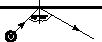
\includegraphics[width=0.6\linewidth]{piljard_joonis.pdf}
  \vspace{-1em}
\end{center}


\yl{Joonlaud koridoris}
Seisad \SI{1}{\m} laiuses koridoris, mille mõlemas seinas on peegel. Peeglite vahel, parempoolsest peeglist \SI{30}{\cm} kaugusel asetseb vertikaalselt kitsas objekt. Sina oled koridoris, käes joonlaud, mida hoiad vertikaalselt enda ees. Märkad, et joonlaua \SI{10}{\cm} näib sulle sama pikk kui objekt ise, \SI{7.5}{\cm} sama pikk kui objekti peegeldus parempoolses peeglis ja \SI{3.75}{\cm} sama pikk kui objekti teine peegeldus parempoolses peeglis. Kui kaugel seisad peeglist?
\punktid{10} \autor{Sandra Schumann}

\yl{Jahtumine}
Sofial on kaks ühesugust koonusekujulist kaaneta termost, mis on osaliselt täidetud võrdse koguse vedelikuga temperatuuril $T=\SI{40}{\celsius}$. Koonusekujulised termosed on asetatud nii, et vedelikupind on põhjaga paralleelne ja koonuse tipp on allpool. Sofia lisab ühte termosesse juurde sama koguse soojemat vedelikku temperatuuril $T_\text{lisa} = \SI{88}{\celsius}$, soojuslik tasakaal saabub hetkeliselt. Seejärel mõõdab Sofia otsekohe vedelike jahtumiskiirust ning leiab, et soojema vedeliku jahtumise kiirus on $k=\num{1.62}$ korda suurem jahedama vedeliku jahtumise kiirusest. Jahtumisvõimsus on võrdeline jahutatava pindala ja temperatuuride vahega. Leidke õhutemperatuur $T_\text{õhk}$. Eeldage, et vedeliku ja termose vahel soojusvahetust ei toimu ning et vedeliku tihedus ei sõltu temperatuurist.

\textit{Vihje}: koonuse ruumala $V=\frac{1}{3}S_p H$, kus $S_p$ on koonuse põhja pindala ning $H$ selle kõrgus.
\punktid{10} \autor{Uku Andreas Reigo}

\newpage
\begin{wrapfigure}[9]{r}{0.1\textwidth}
  \vspace*{-0mm}
  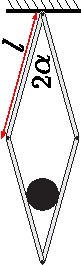
\includegraphics[width = 0.1\textwidth]{rhombus-ball.pdf}
\end{wrapfigure}
\yl{Romb}
Laest ripub rombikujuline liigendiga konstruktsioon, mis on valmistatud massita varrastest pikkusega $l$, vt joonis. Silinder massiga $m$ pannakse rombi sisse. Selle tulemusel võtab romb tasakaaluasendi, kus rombi tipunurk on $2\alpha$. Hõõrdumine silindri ja varda vahel on tühiselt väike. Leidke silindri raadius.
\punktid{12} \autor{Jaan Kalda}

\yl{Kolmnurk}
Koondav lääts fookuskaugusega $f$ tekitab täisnurksest kolmnurgast, mille üks nurk on $\SI{30}{\degree}$ kujutiseks kolmnurga, mis on samuti täisnurkne ja mille üks nurk on  $\SI{30}{\degree}$. Kolmnurga hüpotenuus kulgeb piki läätse optilist peatelge. Leidke kolmnurga hüpotenuusi pikkus.
\punktid{12} \autor{Jaan Kalda}

\yl{Udu}
Kuiva (st ilma igasuguse veeauruta) õhu molaarmass $\mu_a=\SI{28.97}{\g\per\mole}$, vee molaarmass $\mu_v=\SI{18.02}{\g\per\mole}$. Teatud õhurõhu juures on temperatuuril $T_1=\SI{25}\celsius$ kuiva õhu tihedus $\rho_k=\SI{1182.8}{\g\per\m\cubed}$ ning teatud niiske kuid udupiiskadeta õhumassi tihedus $\rho=\SI{1169.3}{\g\per\m\cubed}$. Milline on selle õhumassi tihedus temperatuuril $T_2=\SI{10}\celsius$, kui on teada, et sellel temperatuuril on küllastunud veeauru tihedus $\rho_m=\SI{9.4}{\g\per\m\cubed}$. Eeldage, et kondenseeruvad udupiisad jäävad õhku hõljuma ja et vee tihedus on palju suurem, kui õhu oma.
\punktid{12} \autor{Jaan Kalda}


\begin{wrapfigure}[9]{r}{3cm}
  \vspace*{-5mm}
  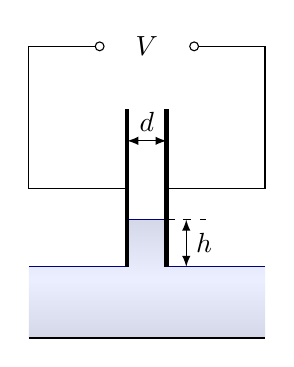
\begin{tikzpicture}
    \colorlet{watercolor}{blue!80!cyan!10!white}
    \tikzstyle{water}=[draw=none, top color=watercolor!90!black!90, bottom color=watercolor!90!black!90, middle color=watercolor!80,shading angle=0]
    \tikzstyle{waterborder}=[draw=blue!50!black]
    \def\l{0.9} % Water height
    \def\L{1.2*\l} % Container height
    \def\W{3} % Container width
    \def\x{0.5} % Capacitor height
    \def\y{2} % Capacitor width
    \def\h{0.6} % Water height in capacitor
    \def\cW{\W} % Circuit width
    \def\cH{0.9*\y} % Circuit height

    % % Circuit
    % \draw(\W/2 + \x/2, \l+\y/2) -- ++(\cW/2 - \x/2, 0) --++ (0, \cH) to[battery1] node[above, pos=0.1]{$V$} ++(-\cW,0) -- ++(0, -\cH) -- (\W/2 - \x/2, \l+\y/2);
    \draw(\W/2 + \x/2, \l+\y/2) -- ++(\cW/2 - \x/2, 0) --++ (0, \cH) --++ (-0.3*\cW, 0) to[open, name=V1, o-o] ++(-0.4*\cW,0) --++ (-0.3*\cW, 0) --++ (0, -\cH) -- (\W/2 - \x/2, \l+\y/2);
    \node  at (V1.center) {$V$};

    % Water
    \draw[water]
    (0,0) -- ++(\W,0) -- ++(0,\l) -- ++(-\W/2 + \x/2,0) -- ++(0,\h) -- ++(-\x,0) -- ++(0,-\h) --  ++(-\W/2+\x/2,0) -- ++(0,-\l);
    \draw[waterborder]
    (0, \l) -- ++(\W/2 - \x/2, 0)
    (\W, \l) -- ++(-\W/2 + \x/2, 0)
    (\W/2 - \x/2, \l + \h) -- ++(\x, 0);

    % Container
    \draw[thick] (0, 0) -- ++(\W,0);

    % Capacitor
    \draw[ultra thick] (\W/2 - \x/2, \l) -- ++(0, \y);
    \draw[ultra thick] (\W/2 + \x/2, \l) -- ++(0, \y);

    % Labels
    \draw[dashed] (\W/2 + \x/2, \l+\h) -- ++(\x,0);
    \draw[latex-latex] (\W/2 + \x, \l) -- ++(0, \h) node[midway,right] {$h$};

    \draw[latex-latex] (\W/2 - \x/2, \l+0.8*\y) -- ++(\x, 0) node[midway,above] {$d$};
  \end{tikzpicture}
\end{wrapfigure}
\yl{Kondensaator vedelikus}
Plaatkondensaator plaatidevahelise kaugusega $d$ on vertikaalasendis ja otsapidi vedelikus nii, nagu näidatud joonisel. Vedeliku dielektriline läbitavus on $\varepsilon$ ja kondensaatori plaatidele on rakendatud pinge $V$. Kui kõrgel $h$ on  plaatide vahelises ruumiosas vedeliku nivoo võrreldes ülejäänud vaba vedeliku pinnaga? Vaakumi dielektriline läbitavus on $\varepsilon_0$, õhu dielektriline läbitavus $\varepsilon_g=1$, vedeliku tihedus on $\rho$ ja vabalangemise kiirendus on $g$. Vedeliku pindpinevusega võib mitte arvestada; kondensaatori kõrgus ja laius ning õhuga täidetud kondensaatoriosa kõrgus on palju suuremad, kui $d$.
\punktid{12} \autor{Konstantin Dukatš}
\begin{center}
\end{center}

\end{document}